\documentclass{webofc}
\usepackage{listings}
\usepackage{minted}
\usepackage{subfig}
\usepackage{hyperref}
\usepackage{graphicx}
\usepackage{subcaption}
\usepackage[utf8]{inputenc}
\usepackage{tikz}

\usepackage[varg]{txfonts}   % Web of Conferences font

\newminted{cpp}{gobble=2, mathescape, numbersep=3pt, frame=lines,escapeinside=||, mathescape, framesep=2mm, baselinestretch=1, fontsize=\scriptsize, linenos=true}
\newmintinline{cpp}{}

\usetikzlibrary{shadows, arrows, fit, positioning, matrix, shapes}
\usetikzlibrary{decorations.markings}

% Define colors
\definecolor{my_yellow}{RGB}{255, 253, 217}
\definecolor{my_orange}{RGB}{255, 127, 0}
\definecolor{my_lightblue}{RGB}{105, 186, 249}
\definecolor{my_purple}{RGB}{150, 154, 219}
\definecolor{my_green}{RGB}{90, 194, 160}

% Define block styles  
\tikzset {
  bigbox/.style = {draw, thick, fill=gray!10, rounded corners, rectangle},
  box/.style = {draw, thick, minimum height=0.8cm, minimum width=1.5cm, rounded corners, rectangle, fill=white, anchor=south},
  model/.style = {draw, thick, fill=white, text centered, minimum height=3em, minimum width=4em, rounded corners, drop shadow},
  user/.style = {draw, thick, ellipse, fill=white, text centered, minimum height=3em, minimum width=5em, drop shadow},
  line/.style = {->, thick, color=black, shorten <=2pt, shorten >=2pt, >=stealth'},
  plain/.style = {minimum width=1em},
  %\draw [line, ->] (m1.north) ++(-15pt,-1pt) arc [start angle=-140, end angle=-400, radius=20pt] node[midway] {$T_{M_1}$} ;
  % This works around an issue with node[midway] http://tex.stackexchange.com/questions/38763/how-to-place-a-node-in-the-middle-of-an-arc                
  arcnode/.style 2 args={
    decoration={
                 raise=#1,             
                 markings,   
                 mark=at position 0.5 with {\node[inner sep=0] {#2};}
            },
            postaction={decorate}
    }
}

% Define the layers to draw the diagram
\pgfdeclarelayer{background}
\pgfdeclarelayer{foreground}
\pgfsetlayers{background,main,foreground}

% Draw background
\newcommand{\background}[5]{%
  \begin{pgfonlayer}{background}
    % Left-top corner of the background rectangle
    \path (#1.west |- #2.north)+(-0.5,0.25) node (a1) {};
    % Right-bottom corner of the background rectanle
    \path (#3.east |- #4.south)+(+0.5,-0.25) node (a2) {};
    % Draw the background
    \path[rounded corners, draw=black!50, dashed, name=box]
      (a1) rectangle (a2);
    \path (a1 |- a2) -- (a2) node[midway,below] {\large\textit{#5}};
  \end{pgfonlayer}}

% Define a circled symbol command used throughout the thesis.
\newcommand*\circled[1]{\tikz[baseline=(char.base)]{
            \node[shape=circle,draw,inner sep=2pt] (char) {#1};}}

\begin{document}

\title{Optimizing Frameworks’ Performance Using C++ Modules Aware ROOT}

\author{\firstname{Yuka}
\lastname{Takahashi}\inst{1,2}
\fnsep\thanks{\email{yuka.takahashi@cern.ch}} \and
        \firstname{Vassil}
        \lastname{Vassilev}\inst{1}\fnsep\thanks
        {\email{vvasilev@cern.ch}}
        \firstname{Oksana}
        \lastname{Shadura}\inst{3}
        \fnsep\thanks{\email{oksana.shadura@cern.ch}}
        \firstname{Raphael}
        \lastname{Isemann}\inst{2,4}
        \fnsep\thanks{\email{isemann@student.chalmers.se}}
}

\institute{Princeton University, Princeton, New Jersey 08544, United States
\and
           CERN, Meyrin 1211, Geneve, Switzerland
\and
           University of Nebraska Lincoln, 1400 R St, Lincoln, NE 68588, United States
\and
           Chalmers University of Technology, Chalmersplatsen 4, 41296 Göteborg, Sweden
}

\abstract{%
The performance of software frameworks for HEP has been a issue for a long time. ROOT is a core framework which is used broadly in HEP and in outside HEP. The performance of Cling C++ interpreter, which serves as a back-end of ROOT consumes large amount of resources when executing ROOT. ROOT was extended with experimental support for using C++ modules during runtime, which is being implemented in Clang with aims to reduce its compilation time. However, within ROOT, compilation time turns into runtime as it's using Cling C++ interpreter. This paper presents the results and challenges with C++ modules in ROOT and its early adoption to CMSSW.

%This paper shows the status of the C++ Modularization in ROOT and CMSSW. It argues for a bottom-up adoption approach and outlines a set of tools to aid the process. The authors share performance results and implementation experience gained from ROOT adaptation of C++ Module and from migrating CMSSW and its dependencies.

%The LLVM community advances its C++ Modules technology providing an io-efficient, on-disk code representation capable of reducing build times and peak memory usage. Significant amount of efforts were invested in teaching ROOT and its toolchain to operate with clang's implementation of the C++ Modules. Currently, C++ Modules files are used by: cling to avoid header re-parsing; rootcling to store io information in a cross-platform way; and ROOT's reflection layer to implement implicit and explicit runtime shared library loading.

%ROOT builds and works with C++ Modules in its dictionary system showing promising performance. The conducted work paved our way for optimizing experiments' software stacks to achieve performance even beyond the observed in ROOT. The new technology adds three new requirements. First, every dictionary header needs to be parsable on its own. Secondly, it should not depend on outside macro definitions which can alter its content. Thirdly, all its direct or indirect includes should be also in a C++ Module. This talk shows the status of the C++ Modularization in ROOT and CMSSW. It argues for a bottom-up adoption approach and outlines a set of tools to aid the process. The authors share performance results and implementation experience gained when migrating CMSSW and its dependencies such as HepMC, Geant and boost.
}
%
\maketitle
%
\section{Introduction}
\label{intro}
This work continues from our previous publication \ref{vassil-paper}. We will give an update from \ref{vassil-paper} and will clarify the contribution of this paper.

C++ Modules technology, gives an efficient serialization, on-disk header representation. Significant amount of efforts were invested in teaching ROOT and its toolchain to operate with clang's implementation of the C++ Modules. Currently, C++ Modules files are used by: cling to avoid header re-parsing; rootcling to store io information in a cross-platform way; and ROOT's reflection layer to implement implicit and explicit runtime shared library loading.

ROOT builds and works with C++ Modules in its dictionary system showing promising performance. The conducted work paved our way for optimizing experiments' software stacks to achieve performance even beyond the observed performance in ROOT. The new technology adds three new requirements. First, every dictionary header needs to be parsable on its own. Secondly, it should not depend on outside macro definitions which can alter its content. Thirdly, all its direct or indirect includes should be also in a C++ Module.

ROOT has several features which interact with libraries and require implicit header inclusion. This can be triggered by reading or writing data on disk, or user actions at the prompt. Often, the headers are immutable and re-parsing is redundant. C++ Modules are designed to minimize the re-parsing of the same header content by providing an efficient on-disk representation of C++ code.

This paper is structured in six sections: section \ref{background}, Background, makes a overview of optimization in current ROOT and gives a comparison with C++ Modules; section \ref{implementation}, Implementation, gives a explanation how we implemented runtime C++ modules in ROOT; section \ref{results}, Results, show the performance results and correctness results which gives a motivation for experiments to start using runtime C++ modules; section \ref{limitationsandfuture}, Limitations and future works, explains the limitation of current implementation and explains future works!

\section{Background}
\label{background}

In this section we will explain the mechanism of three current performance optimizations in ROOT: ROOT precompiled header (PCH), rootmap file (ROOTMAP), and a root file with ROOT I/O optimization information (RDICT) and their drawbacks compared with precompiled modules (PCMs).

\subsection{Existing header parsing implementation: PCH}
\label{pch}

The ROOT precompiled header (PCH) reduces the CPU and memory cost for ROOT’s heavily used libraries. The precompiled header technology is well-understood since decades. It is an efficient on-disk representation of the state of the compiler after parsing a set of headers. It can be loaded before starting the next instance to avoid doing redundant work. At build time, rootcling (ROOT’s dictionary generator) creates one PCH file which is attached at ROOT startup time.

The precompiled modules (PCM) is the file which stores header information which is used by C++ Modules infrastructure. As is shown in \ref{fig:pchandpcm}, the difference of this representation from PCH is that PCM can be created explicitly for each specific headers, with which you can define in module map files. This mechanism makes PCM separable, and in ROOT, one PCM file corresponds to one library.

Major drawback of PCH is the fact that if third-party users want to include their libraries, they have to recompile PCH every time any header file was changed, which becomes an expensive operation. C++ modules solve this drawback, as they are separable by design.

\begin{figure}[!h]
  \centering
  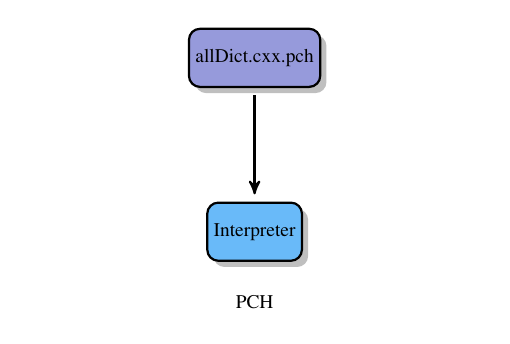
\begin{tikzpicture}[outer sep=0.05cm, node distance=0.8cm, scale=0.7, transform shape]
        
    \node[model, fill=my_purple, name=pch] (pch) {allDict.cxx.pch};
    \node[model, fill=my_lightblue, name=interpreter, below=2cm of pch] (interpreter) {Interpreter};

    \draw[line, ->] (pch.south) -- (interpreter);
    
    \node [below=1cm, align=flush center,text width=8cm] at (interpreter) { PCH };
  \end{tikzpicture}
  \hfill
  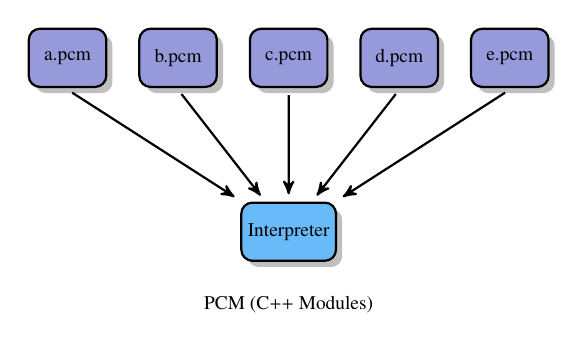
\begin{tikzpicture}[outer sep=0.05cm, node distance=0.8cm, scale=0.7, transform shape]
        
    \node[model, fill=my_purple, name=a] (a) {a.pcm};
    \node[model, fill=my_purple, name=b, right=0.5cm of a] (b) {b.pcm};
    \node[model, fill=my_purple, name=c, right=0.5cm of b] (c) {c.pcm};
    \node[model, fill=my_purple, name=d, right=0.5cm of c] (d) {d.pcm};
    \node[model, fill=my_purple, name=e, right=0.5cm of d] (e) {e.pcm};

    \node[model, fill=my_lightblue, name=interpreter, below=2cm of c] (interpreter) {Interpreter};

    \draw[line, ->] (a.south) -- (interpreter);
    \draw[line, ->] (b.south) -- (interpreter);
    \draw[line, ->] (c.south) -- (interpreter);
    \draw[line, ->] (d.south) -- (interpreter);
    \draw[line, ->] (e.south) -- (interpreter);
    
    \node [below=1cm, align=flush center,text width=8cm] at (interpreter) { PCM (C++ Modules) };

  \end{tikzpicture}
  \caption{Comparison of PCH and C++ Modules in ROOT}
  \label{fig:pchandpcm}
\end{figure}

\subsection{Existing performance optimization in ROOT: ROOTMAP and RDICT}
\label{dictgen}

ROOTMAP files reduce parsing for code which is not in the PCH. RDICT files store some useful information, particularly about class offsets in ROOT files to avoid the potentially expensive call to the interpreter if the information is not the PCH. 

\begin{listing}[h]
    \noindent
    \begin{minipage}[h]{\textwidth}
    \begin{cppcode*}{}
    // Foo.h
        |\label{line:foobar}|namespace foo { struct bar{}; }
        |\label{line:structs}|struct S{};

    // libFoo.rootmap
        |\label{line:decls}|{ decls }
        namespace foo { }
        struct S;
 
        |\label{line:libfoo}|[ libFoo.so ]
        # List of selected classes
        class bar
        struct S

    // G__Foo.cxx (aka libFoo dictionary)
        namespace {
          void TriggerDictionaryInitialization_libFoo_Impl() {
            static const char* headers[] = {"Foo.h"}
            // More scaffolding
            extern int __Cling_Autoloading_Map;
            namespace foo{struct __attribute__((annotate("$clingAutoload$Foo.h"))) bar;}
            struct __attribute__((annotate("$clingAutoload$Foo.h"))) S;
           // More initialization scaffolding.
        }
    \end{cppcode*}
    \end{minipage}
    \caption{C++ header {\it Foo.h} defines {\it foo:bar} and struct S. {\it libFoo.rootmap} contains forward decls and list of classes in order to autoload libraries. {\it G\_\_Foo.cxx} generated to insert forward declaration to ROOT when the {\it libFoo} library was loaded.}
    \label{list:foo}
\end{listing}

ROOT will locate all files with extensions {\it *.rootmap} at its startup time. It parses the code in Line \ref{line:decls} \{decls\} section and creates an internal map for the entities defined in Line \ref{line:libfoo} [libFoo.so] section. Upon seeing an unknown identifier, the implementation searches in the database if this is a known entity.

\begin{listing}[h]
    \noindent
    \begin{minipage}[h]{\textwidth}
    \begin{cppcode*}{linenos=true}
    |\label{line:prompt1}|root [] S *s;           // Does not require a definition.
    |\label{line:prompt2}|root [] foo::bar *baz1; // Does not require a definition.
    |\label{line:prompt3}|root [] foo::bar baz2;  // Requires a definition.
    \end{cppcode*}
    \end{minipage}
    \caption{Psuedo ROOT prompt which shows the efforts which ROOT does to avoid parsing redundant code. S is defined in Line \ref{line:structs} in Listing \ref{list:foo} and {\it foo::bar} is defined in Line \ref{line:foobar} in Listing \ref{list:foo}.}
    \label{list:prompt}
\end{listing}

\begin{listing}[h]
    \noindent
    \begin{minipage}[h]{.7\textwidth}
    \begin{cppcode*}{}
    root [] namespace foo { }; struct S;
    root [] S *s;
    \end{cppcode*}
    \end{minipage}
    \caption{Pseudo ROOT prompt which is functionally equivalent to taking a pointer of Struct S. (Line \ref{line:prompt1} in Listing \ref{list:prompt})}
    \label{list:line1}
\end{listing}

Line \ref{line:prompt1} in Listing \ref{list:prompt} does not require a definition and the forward declaration consumed at the initialization time is sufficient, so the parsing of {\it Foo.h} is not required. The behavior of Line \ref{line:prompt1} in Listing \ref{list:prompt} is equivalent to Listing \ref{list:line1}.

\begin{listing}[h]
    \noindent
    \begin{minipage}[h]{.7\textwidth}
    \begin{cppcode*}{}
    |\label{line:line2beggining}|root [] namespace foo { }; struct S;
    root [] foo::bar /*store parsing state*/
        gSystem->Load("Foo");
        // More scaffolding.
        extern int __Cling_Autoloading_Map;
        namespace foo{struct __attribute__((annotate("$clingAutoload$Foo.h"))) bar;}
        struct __attribute__((annotate("$clingAutoload$Foo.h"))) S;
        // More initialization scaffolding.
        |\label{line:beforerestoreparsing}|/*restore parsing state*/ *baz1;
        
        |\label{line:restoreparsing}|#include <Foo.h>/*restore parsing state*/;
    \end{cppcode*}
    \end{minipage}
    \caption{Pseudo code which Line \ref{line:line2beggining} to Line \ref{line:beforerestoreparsing} is functionally equivalent to Line \ref{line:prompt2} in Listing \ref{list:prompt}. Line \ref{line:line2beggining} to Line \ref{line:restoreparsing} is functionally equivalent to Line \ref{line:prompt3}}
    \label{list:line2}
\end{listing}

Line \ref{line:prompt2} also does not require a definition. However, the second identifier lookup fails. ROOT knows that {\it foo::bar} is in {\it libFoo} by the information from rootmap files (Line \ref{line:libfoo}). It dlopens {\it libFoo} which in turn, during its static initialization, inserts annotated forward declaration as shown in {\it G\_\_Foo.cxx}. This resolves {\it foo::bar} which avoids the parsing of {\it Foo.h} at relatively small overhead.
The loading of the annotated forward declarations can happen at any time during parsing. This is so-called "recursive parsing" and is a code path that exists only in ROOT, and is not exercised by clang itself. The behavior of Line \ref{line:prompt2} is equivalent to Listing \ref{list:line2}.

Line \ref{line:prompt3} requires a definition and the implementation behaves exactly as in Line \ref{line:prompt2}. Then it is informed that a definition is required, it reads the information in the annotation and parses {\it Foo.h} as is shown in Line \ref{line:restoreparsing}. The recursive parsing happens at two places making this code path error prone.

To recap, ROOTMAP require a lot of maintenance and goes on an untested codepath, while RDICT has a limited scope of optimization. The two features require a lot of mechanisms to work together and there are noticeable corner cases.

\section{Implementation}
\label{implementation}

An implementation of the C++ modules concept itself exists in the LLVM frontend Clang which is used as a library by ROOT. Clang supports the Modules TS and hosts modules research and development work. The implementation encourages incremental, bottom-up adoption of the modules feature. Modules in Clang are designed to work for C, C++, ObjectiveC, ObjectiveC++ and Swift. Users can enable the modules feature without modifications in header files. The LLVM compiler allows users to specify module interfaces in dedicated file, called module maps files. A module map file expresses the mapping between a module file and a collection of header files. If the compiler finds such file in the include paths it automatically generates, imports and uses module files. The module map files can be mounted using the compiler’s virtual file system overlay mechanism to non-writable production library installations. In practice, a non-invasive modularization can be done easily by introducing a module map file. In a number of cases the module map files can be automatically generated if the build system knows about the list of header files in every package.

Several steps were taken to adopt C++ modules in ROOT. First, we supported compile-time C++ modules with Clang, which {\it compiles} ROOT with modules aware Clang. It improves ROOT compilation two times, and this effort includes generating module map files and resolving cyclic header dependency inside ROOT. Next, we taught rootcling dictionary generator to generate pcm files attached with I/O information. We taught ROOT to preload all pre-generated pcm at startup time, in order to make declaration available without \#including the appropriate headers. Also we implemented autoloading of libraries in ROOT which are not depending on old infrastructure (ROOTMAPS), which gives correctness benefits shown in section \ref{correctness} and is surprisingly efficient compared to ROOTMAPS. This is because we can infer the library name from pcm name. Beyond that we have done a huge amount of performance optimization in ROOT and in Clang.

For C++ modules adoption in experiments, we have been working closely with CMSSW team. Already, ROOT can be compiled with runtime C++ in CMS enviroment, and we will enable pcm generation for their libraries one by one. We can gradually migrate dictionary generation to pcm, as our current implementation fall back to ROOTMAP when pcm is not generated. This enables us incremental migration from old to new infrastructure.

\subsection{Preloading of allmodules}
\label{subsec:preloading}

C++ Modules-aware ROOT preloads all modules at start up time. Listing \ref{list:prompt} becomes equivalent to Listing \ref{list:implicit-include}.

\begin{listing}[h]
    \noindent
    \begin{minipage}[h]{.7\textwidth}
    \begin{cppcode*}{}
    |\label{line:importroot}|root [] import ROOT.*;
    |\label{line:importfoo}|root [] import Foo.*;
    root [] foo::bar *baz1;
    \end{cppcode*}
    \end{minipage}
    \caption{Pseudo ROOT prompt to show the example of implicit \#include. {\it foo::bar} can be used without even \#including foo.h. With modules, this feature is supported by importing all modules at the startup time, as shown in Line \ref{line:importroot} and \ref{line:importfoo}.}
    \label{list:implicit-include}
\end{listing}

This implementation avoids recursive actions and relies on a well-defined (by the C++ standard) behavior. Currently, this comes with a constant performance overhead which we go in details in section \ref{performance}.

\subsection{Autoloading support in Runtime C++ modules}
\label{subsec:autoloading}

\begin{listing}[h]
    \noindent
    \begin{minipage}[h]{\textwidth}
    \begin{cppcode*}{}
    // A.h
        #include <string>
        #include <vector>
        template <class T, class U = int> struct AStruct {
          void doIt() { /*...*/ }
          std::string Name; 
          std::vector<U> Collection;
        };

        template<class T, class U = AStruct<T>>
        inline void freeFunction() { /* ... */ }
        inline void do(unsigned N = 1) { /* ... */ }
    
    // Main.cpp
        #include "A.h"
        int main() {
          do();
          return 0;
        }
        
    // ROOT prompt
        root [] AStruct<float> S0;     // Implicit loading of libA. Full descriptor required.
        root [] AStruct<float>* S1;    // Implicit loading of libA. No full descriptor required.
        root [] if (gFile) S1->doIt(); // Implicit loading of libA. Full descriptor required.
        root [] gSystem->Load("libA"); // Explicit loading of libA. No full descriptor required.
        |\label{line:implicitloading}|root [] do();                  // Error: implicit loading of libA is currently unsupported.
    \end{cppcode*}
    \end{minipage}
    \caption{Example of ROOT prompt in order to explain ROOT library loading mechanism. {\it Main.cpp}, reuses code from {\it libA} by including {\it libA}’s descriptor and links against {\it libA}. The full descriptor can contain thousands of files expanding to millions of lines of code. This pattern is not only used in the ROOT prompt but in I/O hotspots such as {\it ShowMembers} and {\it TClass::IsA}.}
    \label{list:autoloadingprompt}
\end{listing}

Currently, ROOT’s lack of support of Line \ref{line:implicitloading} in Listing \ref{list:autoloadingprompt} is a long-standing, known limitation that is lifted with modules.

A naive implementation of this feature would require inclusion of all reachable library descriptors (aka header files) at ROOT startup time. Of course this is not feasible and ROOT inserts a set of optimizations to fence itself from the costly full header inclusion. Unfortunately, several of them are home-grown and in a few cases inaccurate (eg Line \ref{line:implicitloading}) causing a noticeable technical debt.

With runtime C++ modules, it iterates through libraries found in LD\_LIBRARY\_PATH until it finds the definition of currently searching mangled name. This overhead is extremely low as it's only looking into 64 bytes hash in the library to determine whether this library likely has a definition or not, which is called bloom filter.

\section{Results}
\label{results}

\subsection{Performance Results}
\label{performance}

\begin{figure}
\centering
    \begin{minipage}{.48\textwidth}
    \subfloat[] {\label{fig:perfBuildingROOT:a} 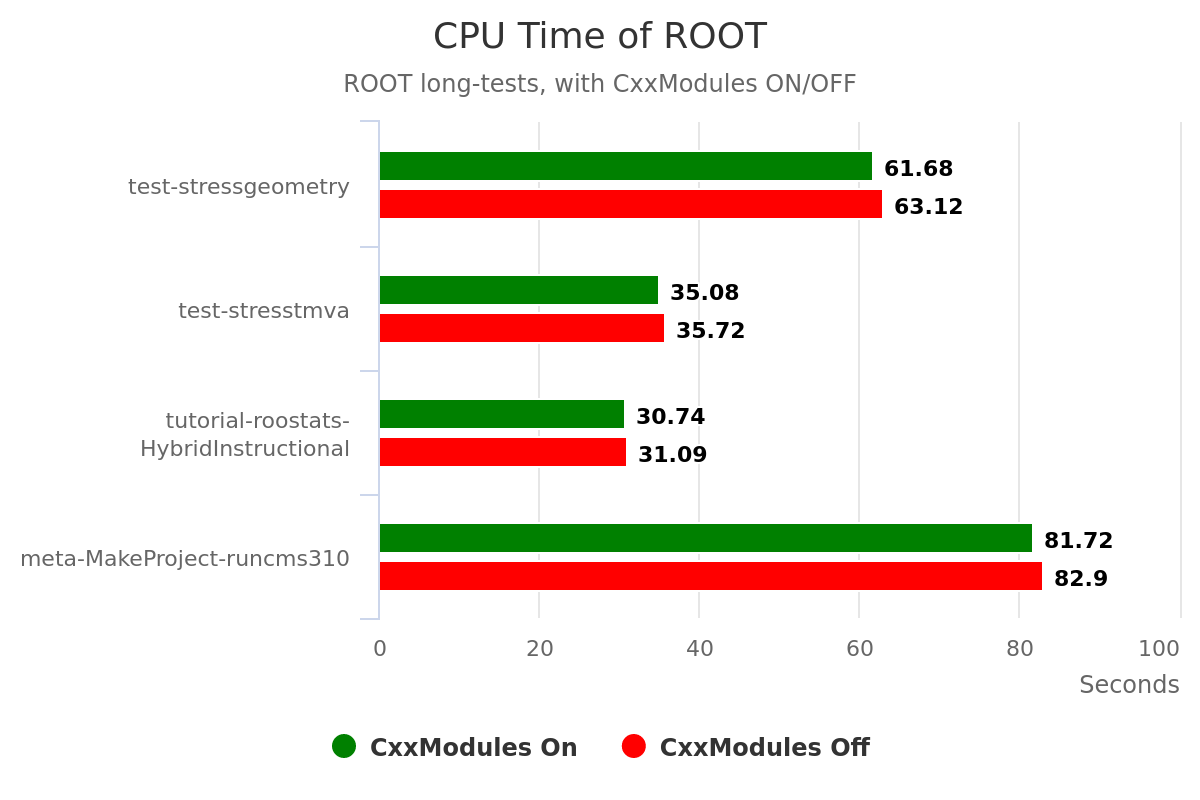
\includegraphics[width=\textwidth]{Long_CPU.png}}
   \end{minipage}\hfill
    \begin{minipage}{.48\textwidth}
    \subfloat[] {\label{fig:perfBuildingROOT:a} 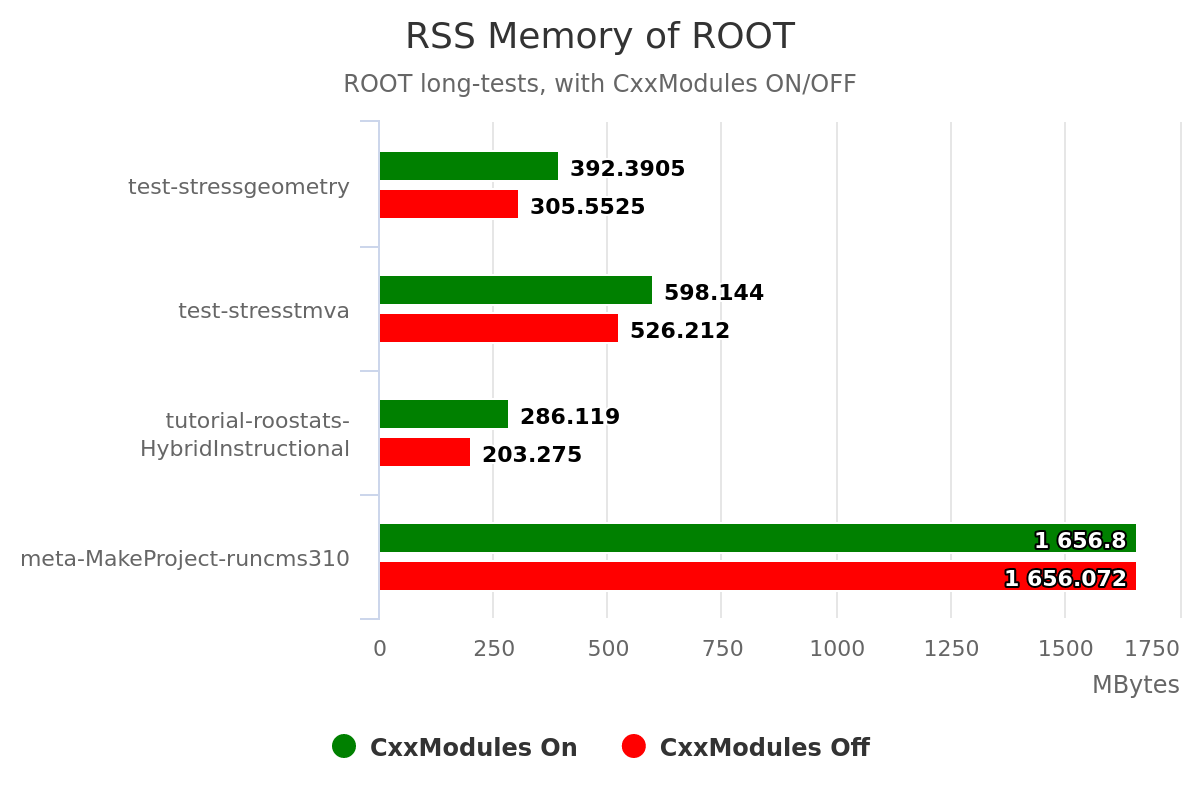
\includegraphics[width=\textwidth]{Long_RSS.png}}
   \end{minipage}
   
    \begin{minipage}{.48\textwidth}
    \subfloat[] {\label{fig:perfBuildingROOT:a} 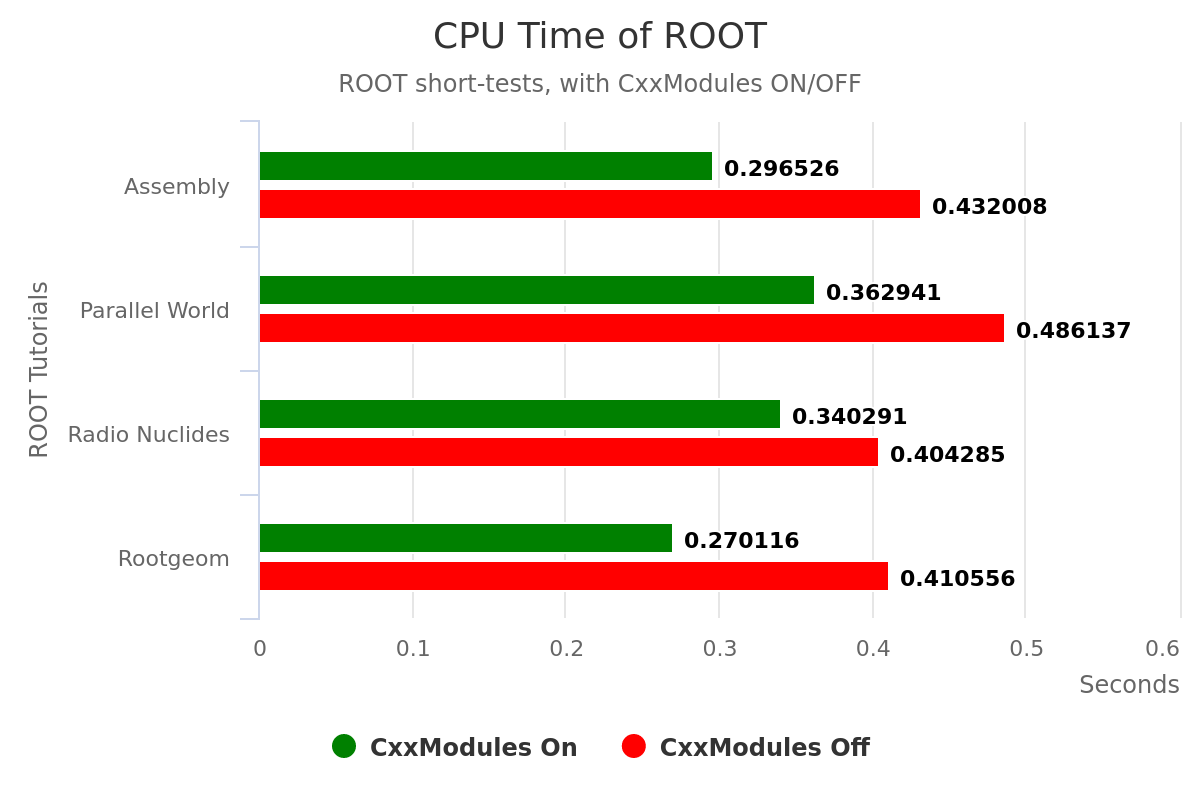
\includegraphics[width=\textwidth]{Short_CPU.png}}
   \end{minipage}\hfill
    \begin{minipage}{.48\textwidth}
    \subfloat[] {\label{fig:perfBuildingROOT:a} 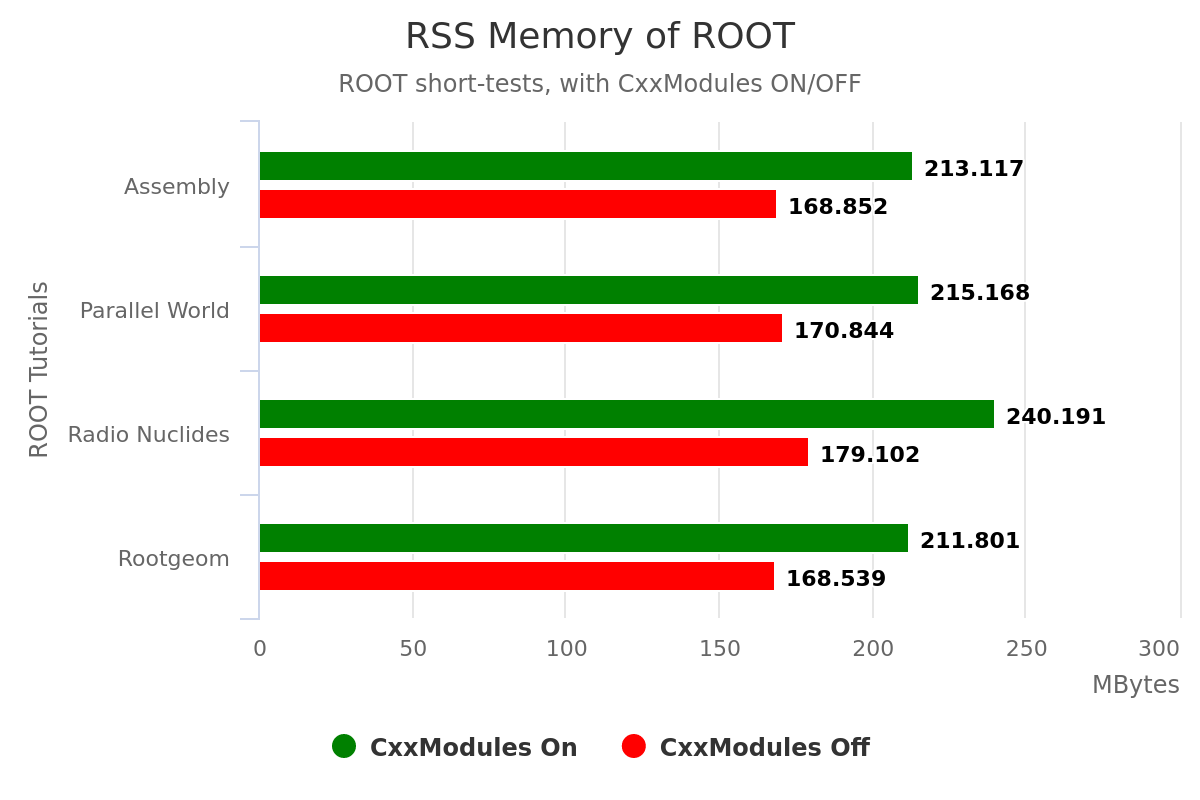
\includegraphics[width=\textwidth]{Short_RSS.png}}
   \end{minipage}
\caption{Performance results: (a), (c) are the measurement of CPU time. (b), (d) are the measurement of RSS. (a), (b) are measuring long tests (over 30 seconds) in ROOT with and without runtime C++ modules. (c), (d) are measuring short tests which is not PCH-nized.}
\label{fig:performance1}
\end{figure}

\begin{figure}
\centering
    \begin{minipage}{.48\textwidth}
    \subfloat[] {\label{fig:perfBuildingROOT:a} 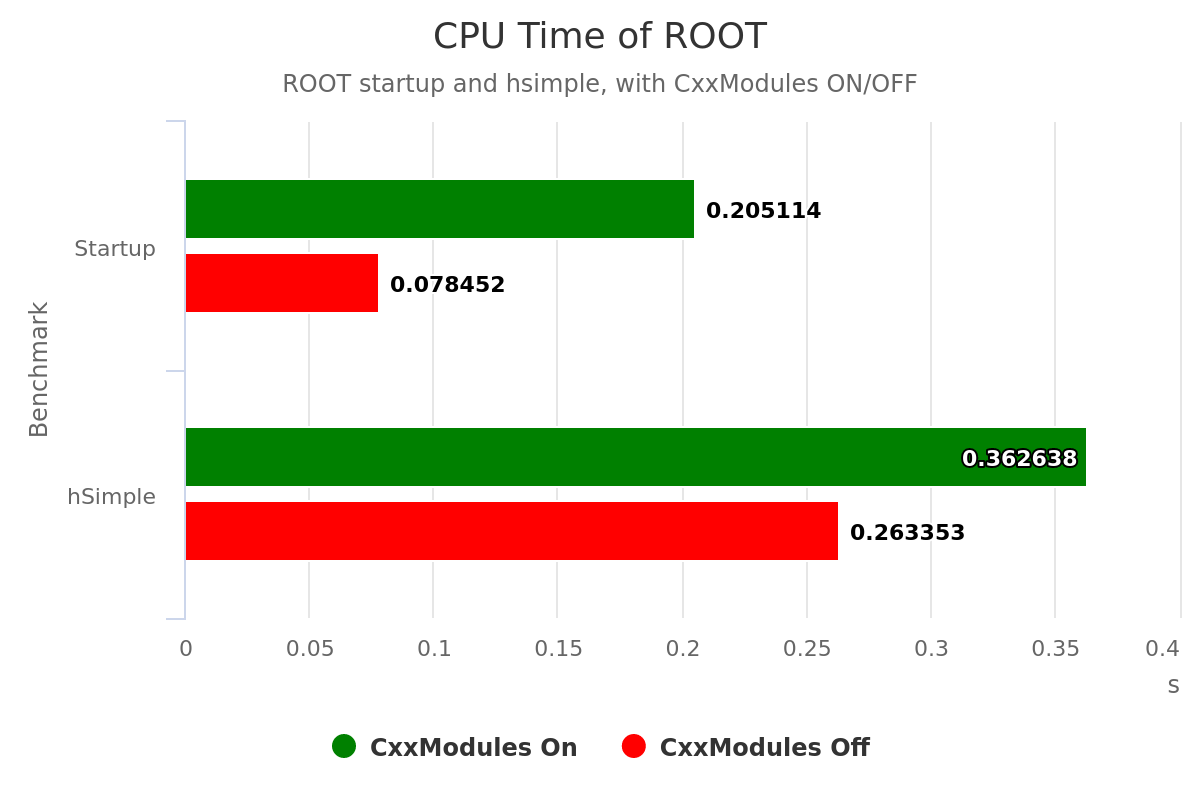
\includegraphics[width=\textwidth]{Startup_CPU.png}}
   \end{minipage}\hfill
    \begin{minipage}{.48\textwidth}
    \subfloat[] {\label{fig:perfBuildingROOT:a} 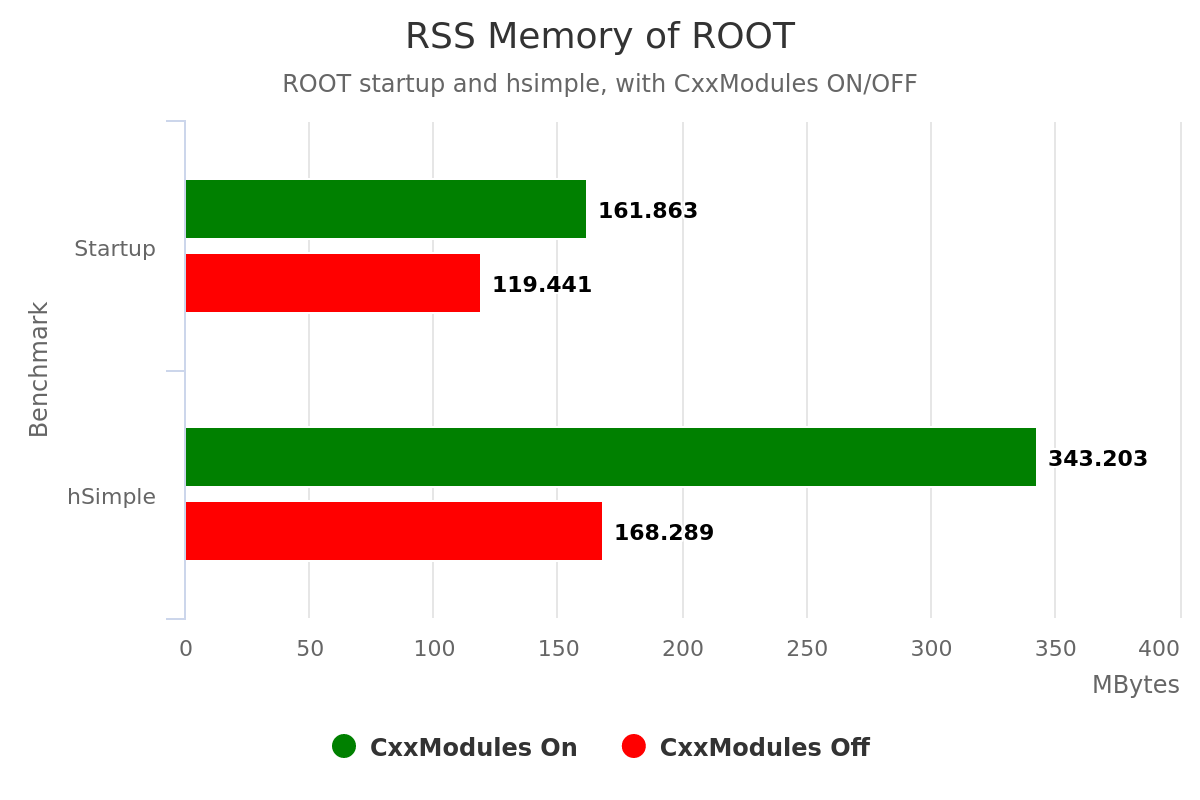
\includegraphics[width=\textwidth]{Startup_RSS.png}}
   \end{minipage}
\caption{Performance results: (a), (b) are the startup time of ROOT and hsimple tutorial, which are the basic benchmarks.}
\label{fig:performance2}
\end{figure}

Figure \ref{fig:performance1} and Figure \ref{fig:performance2} are the performance results we receive from modules, compared to PCH and textual headers which is synthetic benchmarks close to the experiment software stacks.

(a), (c) in Figure \ref{fig:performance1} and (a) in Figure \ref{fig:performance2} are measuring CPU time of ROOT. On the other hand, (b) (d) in Figure \ref{fig:performance1} and (b) in Figure \ref{fig:performance2} are measuring RSS of ROOT.

(a), (b) in Figure \ref{fig:performance1} are testing ROOT longtests, which takes more then 30 seconds. (c), (d) in Figure \ref{fig:performance2} are testing short tests which are not in PCH, which means that they are still using textual include. Thus from those tests we can get a rough assumption of the performance result we will get from modularizing experiments. Figure \ref{fig:performance2} is measuring the startup of ROOT and hsimple tutorial, to show the actual startup time overhead we have from preloading pcms.

The RSS memory regression which can be seen in Figure \ref{fig:performance1} (d) and in Figure \ref{fig:performance2} (b) are mostly due to importing all C++ Modules at the startup. RSS overhead are seen in correspondence of the number of preloaded modules. The startup time overhead is between 40-60 MB depending on the concrete configuration. However, when the workload increases (Figure \ref{fig:performance1} (b)) we notice that the overall memory performance decreases in number of cases.

The CPU time regression in Figure \ref{fig:performance2} (a) and in Figure \ref{fig:performance1} (c) are also due to importing all pcms at the startup. However, in Figure \ref{fig:performance1} (a) C++ modules are doing better than PCH by 1 or 2 seconds. It shows that C++ modules can perform better when the workload of the users' code increases.

The performance of the technology preview is dependent on many factors such as configuration of ROOT and workflow. We also implemented a continuous performance monitoring tool \cite{rootbench} where we compare the performance of the technology preview with respect to standard ROOT.

\subsection{Correctness and extra usability features}
\label{correctness}

\begin{listing}[h]
    \noindent
    \begin{minipage}[h]{.48\textwidth}
    \begin{cppcode*}{}
    root [] gMinuit // Cannot load variable
    IncrementalExecutor::executeFunction:
    symbol 'gMinuit' unresolved while
    linking [cling interface function]!
    \end{cppcode*}
    \end{minipage}\hfill
    \begin{minipage}[h]{.48\textwidth}
    \begin{cppcode*}{}
    root [] gMinuit // Could load libMinuit
    (TMinuit *) nullptr
    \end{cppcode*}
    \end{minipage}
    \caption{Correctness results: Left hand side is ROOT without runtime C++ modules, which cannot autoload extern global variables such as gMinuit. Right hand side is ROOT with runtime C++ modules, with which gMinuit can be autoloaded.}
    \label{list:gMinuit}
\end{listing}

Runtime C++ modules are supporting more features than PCH. As shown in \ref{list:gMinuit}, gMinuit is an extern variable which cannot be autoloaded by ROOT at the moment. However, with modules, we can automatically resolve symbols and cases like those are now correctly handled.

\begin{listing}[h]
    \noindent
    \begin{minipage}[h]{.48\textwidth}
    \begin{cppcode*}{}
    root [] #include <m17n-core.h> // System header
    root [] m17n_init_core()
    IncrementalExecutor::executeFunction:
    symbol 'm17n_init_core' unresolved while
    linking [cling interface function]!
    \end{cppcode*}
    \end{minipage}\hfill
    \begin{minipage}[h]{.48\textwidth}
    \begin{cppcode*}{}
    root [] #include <m17n-core.h> // System header
    root [] m17n_init_core() // Autoload system library
    root []
    \end{cppcode*}
    \end{minipage}
    \caption{Autoloading of system libraries: This is a new feature introduced by runtime C++ modules library autoloading mechanism.}
    \label{list:gMinuit}
\end{listing}

As already noted in section \ref{implementation}, Modules autoloading implementation iterate through LD\_LIBRARY\_PATH which includes system libraries.

\section{Limitations and future works}
\label{limitationsandfuture}

In this section, we will show our limitations and future work.

First, Clang have a limitation in overwriting an outdated pcm file. That is, when building ROOT, modifying the source code and rebuilding might not work. In order to fix this problem, we need to teach Clang to overwrite outdated pcm. It is possible to work around this issue by removing all pcm files in the \$ROOTSYS/lib folder.

Relocatability issues: we have fixed a few of the relocatability issues we
found. We are aware of an obscure relocatability issue when ROOT is copied in another folder and we are rebuild. ROOT picks up both modulemap files in seemingly distinct locations.

Building pcms with rootcling: in rare cases there might be issues when building pcm files with rootcling. The easiest will be to open a bug report to clang, however, reproducing a failure outside of rootcling is very difficult at the moment.

Runtime modules are still an experimental feature. Our ultimate goal is to make it default in ROOT and in experiments:

In addition to above limitations, our ultimate goal is to make this feature default in ROOT. For this, we will give a support to experiments such as CMSSW, and will continue optimizing the performance.

\section{Acknowledgments}

This work has been supported by an Intel Parallel Computing Center grant, by U.S. National Science Foundation grants PHY-1450377 and PHY-1624356, and by the U.S. Department of Energy, Office of Science.

The authors would like to thank CERN/EP-SFT and the ROOT team in particular.

\begin{thebibliography}{}

\bibitem{vassil-paper}
Vassil Vassilev, J. Phys.: Conf. Ser. \textbf{898}, 072023 (2017)

\bibitem{clang-modules-doc}
Clang Modules Documentation, \url{http://clang.llvm.org/docs/Modules.html}, accessed: 2018-24-11

\bibitem{Moduralize-doc}
Modularize Documentation, \url{http://clang.llvm.org/extra/modularize.html}, accessed: 2018-24-11

\bibitem{Gregor-cppcon}
Gregor D,   2016 Modules cppCon, URL \url{http://llvm.org/devmtg/2012-11/#talk6}

\bibitem{Klimek-cppcon}
Klimek M 2016 Deploying C++ Modules to 100s of Millions of Lines of Code cppCon, URL \url{https://cppcon2016.sched.com/event/7nM2/deploying-c-modules-to-100s-of-millions-of-lines-of-code}

\bibitem{Smith-cppcon}
Smith R 2016 There and Back Again: An Incremental C++ Modules Design cppCon, URL \url{https://cppcon2016.sched.com/event/7nM6/there-and-back-again-an-incremental-c-modules-design}

% It's not public yet
% \bibitem{Richards' latest modules TS}
% Richards' latest modules TS

\bibitem{David-talk}
David Blaikie 2018 Build Impact of Explicit and C++ Standard Modules, URL \url{https://youtu.be/b-iiA18BRCQ}

% MEMO: Cite Oksana's paper
\bibitem{rootbench}
Oksana Shadura 2018 Continuous performance monitoring..

% Probably cite CMSSW

\end{thebibliography}

\end{document}

% end of file template.tex



% Notes

<div id='footer'><table width='100%'><tr><td class='right'><a href='http://fusioninventory.org/'><span class='copyright'>FusionInventory 9.1+1.0 | copyleft <img src='/glpi/plugins/fusioninventory/pics/copyleft.png'/>  2010-2016 by FusionInventory Team</span></a></td></tr></table></div>

